%%% Fiktivní kapitola s ukázkami tabulek, obrázků a kódu

\chapter{Simulátor}
Součástí bakalářské práce bylo také naprogramování simulátoru mapy, její vizualizace, implementace všech EA, vše v jazyce C\#. Veškeré informace o simulátoru a jeho součástech můžete najít v dokumentaci na přiloženém CD. V této kapitole popíši pouze spuštění, základní objekty simulátoru a aplikované optimalizace. \par 
\paragraph{Části simulátoru}
\begin{itemize}
	\item \textit{SwarmSimFramework.exe} - konzolová aplikace, která obsahuje kód pro EA optimalizaci a simulaci mapy
	\item \textit{SwarmSimVisu.exe} - program pro vizualizaci, implementovaný ve WPF a C\# 
\end{itemize}

\section*{Spuštění}
Pro spuštění optimalizace SwarmSimFramework.exe je potřeba soubor s konfigurací experimentu, soubory s konfigurací pro ES mají koncovku \textit{.es} a v případě diferenciální evoluce \textit{.expe}. Jednotlivým EA také odpovídají očekávané argumenty. 
\begin{itemize}
	\item evoluční strategie - \textit{SwarmSimFramework.exe -es konfigurace.es}  
	\item diferenciální evoluce - \textit{SwarmSimFramework.exe -de konfigurace.expe} 
\end{itemize}
\par 
V rámci konfiguračních souborů můžeme nastavit charakteristiky mapy, ohodnocení jednotlivých složek fitness, specifikovat druh či počet robotů, název experimentu a název složky s výstupem. Výstupní složka obsahuje serializované nejlepší jedince vždy po 10 generacích, metadata pro graf (číslo generace, hodnoty fitness), serializované veškeré jedince po 100 generacích. V případě ES mají jedinci svou vlastní podsložku z implementačních důvodů (paralelismus). Populace z poslední generace je ještě serializována do složky spuštění. Do konzole, pak program vypisuje základní informace o aktuální generaci.
\par 
Pokud si chceme prohlédnout některé z chování vizuálně, spustíme program SwarmSimVisu.exe. Kde je připraveno grafické rozhraní, kde pomocí tlačítek navolíme vybraný scénář, nastavení mapy a soubory se serializovaným řízením robota. Poté je možné danou simulaci spouštět a zastavovat, při zastavené simulaci pravým klikem na robota lze zobrazit jeho podrobné informace.
\clearpage
\section*{Optimalizace}
Simulace mapy patří mezi časově nejvíce náročnou část. Pro její zrychlení jsem použil paralelního programování, jeho přístup se liší podle EA. Za použití profileru jsem nalezl, že nejvíce času simulace zabralo počítání jednotlivých průsečíků pro senzory, efektory a entity samotné. Pro optimalizaci počtu průsečíků jsem implementoval vlastní datovou strukturu \textit{SpatialHash}. 
\par 
SpatialHash rozděluje mapu na sít malých čtverečků. Každá entita (mimo roboty) je uvedena ve všech čtverečcích do kterých zasahuje. Pro počítání kolizí dostane potenciálně kolidující těleso od SpatialHash množinu obsahující všechny entity zasahujících do stejných čtverečků jako potenciálně kolidující těleso. Jedinou vyjímku tvoří roboti, neboť se často přesouvají po mapě a ve SpatialHash by neustále měnili pozici. Operace spojené s častým pohybem byly více náročné než počítat průsečíky se všemi roboty, takže roboti jsou uloženi v klasickém listu.
\par
Kvůli dalšímu zrychlení jsem se rozhodl použít paralelního běhu programu. Kde se použití paralelismu liší na základě použitých EA. Zatímco v ES lze paralelně zpracovávat každého jedince zvlášť, protože nepotřebuje v evolučních operátorech celou populaci, tak v diferenciální evoluci je potřeba, aby pro každý evoluční operátor byla k dispozici celá generace rodičů. Tím pádem ES můžeme od sebe oddělit jednotlivé jedince a nemusí sdílet žádnou paměť. U diferenciální evoluce bylo rozdělení poněkud složitější, protože v rámci běhu vybírá náhodně z celé populace. Rozhodl jsem se, že oddělím simulace mapy, která probíhá pro nově vzniklého potomka a na její základě se hodnotí jeho fitness. Takže pro každého člena původní populace vznikne nezávislý proces, který vybere z aktuální populace 3 jedince (pouze čtení) a pak nově vzniklého jedince vloží do thread safe datové struktury (list z knihovny System.Collections.Concurrent). Po dokončení všech procesů se přejde k další generaci. Použití paralelního zpracovaní znemožňuje přesné zopakování experimentů, zkoušel jsem experimenty pouštět na rozličných strojích a výsledky řádově odpovídají.  
\clearpage
\section*{Použití}
Pro jednotlivé objekty na mapě jsem vytvořil obecný objektový návrh, který umožňuje jednoduché přidání vlastních objektů, případně používat pouze simulaci na mapě pro jiné účely než optimalizaci chování robotů, či implementací nových evolučních algoritmů.
\par
Celá simulace probíhá v rámci instance třídy Map, ve které se nacházejí všechny objekty figurující v simulaci. Jedná se o překážky, materiály určené ke zpracování, roboty atd. Přesný strom dědičnosti je uveden v dokumentaci. Roboti používaní v experimentech v kapitole \ref{chap:experimenty} mají podobnou základní stavbu. Její hlavní části ilustruje obrázek \ref{obr03:robotModel}, červeně je označeno tělo robota, modrý kruh je rádiový přijímač, černé úsečky představují vzdálenostní senzory, šedivě stínované obdélníky zobrazují kolečka (ve vizuálním programu se nezobrazují).
\par 
Všichni mnou používaní roboti jsou poháněni dvou kolovým motorem. Pro interakci se svět jim slouží efektory (mění prostředí) a senzory (snímají prostředí), v obou případech mají buď podobu úsečky nebo kruhu.
\par
 Mezi modelové úsečkové senzory patří vzdálenostní senzory, který vrací typ a vzdálenost k objektu kolidující se senzorem, typicky mají roboti 3 tyto senzory vpředu. Jako zástupce kruhovitých senzorů můžeme považovat rádiový přijímač, který vrací robotovi ve vektoru intenzitu signálů, které proťaly jeho kruhovou reprezentaci.
 \par 
 Efektory pracují na podobném principy jen místo čtení hodnot z prostředí očekávají vstupní hodnoty s nastavením. Například efektor zpracovávající stromy na dřevo má podobu úsečkového efektoru, pro zpracování musí kolidovat s entitou stromu a na vstupu musí dostat povel pro aktivaci. 
 \begin{figure}[h]\centering
	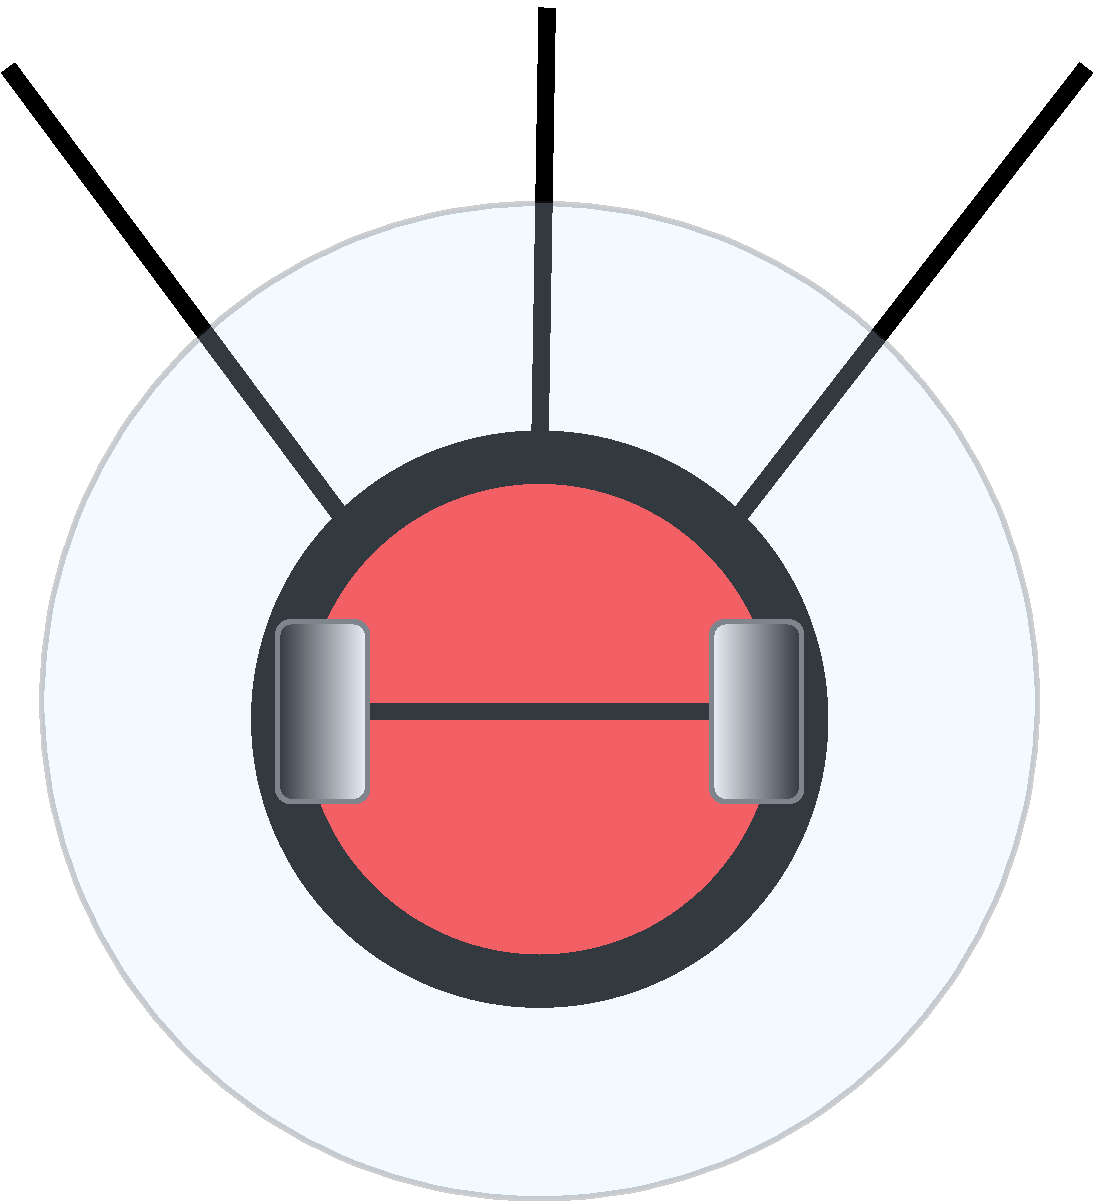
\includegraphics[scale=0.3]{../img/RobotModel}
	\caption{Ilustrativní obrázek obecného robota}
	\label{obr03:robotModel}
\end{figure}
